\appendix


\chapter{\emph{Source code} program}

\section{main.py}
\begin{lstlisting}[language=Python, basicstyle=\tiny]
import sys
from image_editing import ImageEditing
from tkinter import *
from grabcut import GrabCut
from PIL import Image, ImageTk, ImageMath, ImageDraw
import numpy as np

if __name__ == '__main__':
    root = Tk()
    category = "luka_hitam"
    img_name = "2"
    extension = ".jpg"
    image_path = "dataset_3/"+category+"/"+img_name+extension
    tools = ImageEditing(root, image_path, img_name, category)
    root.mainloop()
\end{lstlisting}

\section{image\_editing.py}
\begin{lstlisting}[language=Python, basicstyle=\tiny]
import sys
import os
from tkinter import *
from grabcut import GrabCut
from PIL import Image, ImageTk, ImageMath, ImageDraw
import numpy as np

COLOR = {
    'red' : [0, 0, 255],
    'white' : [255, 255, 255],
    'black' : [0, 0, 0],
    'yellow' : "#FFFF00"
}

F_BG = 0
F_FG = 1
F_PR_FG = 2

KOTAK = {
    "coord" : (),
    "pos" : None,
    "titik_start" : None,
    "titik_akhir" : None,
    'is_init' : False,
    'is_drawn' : False,
}

BRUSH = {
    "size" : 3,
    'is_init' : False,
    'is_drawn' : False,
}

class ImageEditing:
    def __init__(self, root, image_path, image_name, category):
        self.root = root
        self.root.title("Image Segmentation using Grabcut")   
        self.image_path = image_path    
        self.image_name = image_name
        self.category = category

        # Create a frame for title labels
        self.title_frame = Frame(self.root)
        self.title_frame.pack(side=TOP, fill=X)

        # Create a frame for canvases
        self.canvas_frame = Frame(self.root)
        self.canvas_frame.pack(side=TOP, fill=BOTH, expand=YES)  # Adjusted to fill both X and Y, expand

        # Create a frame for buttons
        self.button_frame = Frame(self.root)
        self.button_frame.pack(side=BOTTOM, fill=BOTH)

        # Laod image
        self.image = Image.open(self.image_path)

        # Resize ukuran gambar
        self.setSizeImg() 
        self.image = self.image.resize((new_width, new_height)) # <-- untuk resize ukuran

        self.gambar = np.array(self.image)
        self.gambar2 = self.gambar.copy()
        print("ukuran gambar: ", self.gambar.shape)

        # buat masking dari gambar awal
        self.mask = np.zeros(self.gambar2.shape[:2], dtype=np.uint8)
        self.mask2 = self.mask.copy()

        self.LoadCanvas()

    def LoadCanvas(self):    
        # Make image as main canvas
        main_title_label = Label(self.title_frame, text="Main Canvas", font=('Helvetica', 10, 'bold'))
        self.photo = ImageTk.PhotoImage(self.image)
        self.main_canvas = Canvas(self.canvas_frame, width=self.image.width, height=self.image.height)
        self.main_canvas.create_image(0, 0, anchor=NW, image=self.photo)

        # Create mask canvas
        mask_title_label = Label(self.title_frame, text="Mask Canvas", font=('Helvetica', 10, 'bold'))
        self.mask_image = Image.fromarray(self.mask)
        self.mask_image = self.mask_image.resize((new_width, new_height)) # <-- untuk resize ukuran
        self.mask_photo = ImageTk.PhotoImage(self.mask_image)
        self.mask_canvas = Canvas(self.canvas_frame, width=self.image.width, height=self.image.height)
        self.mask_canvas.create_image(0, 0, anchor=NW, image=self.mask_photo)

        # Create a result canvas for result display
        result_title_label = Label(self.title_frame, text="Result Canvas", font=('Helvetica', 10, 'bold'))
        self.result_image = Image.new("RGB", (self.image.width, self.image.height))
        self.result_photo = ImageTk.PhotoImage(self.result_image)
        self.result_canvas = Canvas(self.canvas_frame, width=self.image.width, height=self.image.height)
        self.result_canvas.create_image(0, 0, anchor=NW, image=self.result_photo)

        
        # Create the buttons with custom styles
        self.draw_rect_button = Button(self.button_frame, text="Draw Rectangle", command=self.drawing_rectangle, bg='#4CAF50', fg='white', font=('Helvetica', 10))
        self.segmentation_button = Button(self.button_frame, text="Segmentation Grabcut", command=self.segmentation_image, bg='#2196F3', fg='white', font=('Helvetica', 10))
        self.save_button = Button(self.button_frame, text="Save Result", command=self.save_result_image, bg='#FFC107', fg='black', font=('Helvetica', 10))
        self.reset_button = Button(self.button_frame, text="Restart Program", command=self.reset_image, bg='#607D8B', fg='white', font=('Helvetica', 10))
        
        # Display canvas
        self.main_canvas.pack(side=LEFT)
        main_title_label.pack(side=LEFT, padx=(10, 220))
        self.mask_canvas.pack(side=LEFT)
        mask_title_label.pack(side=LEFT, padx=(10, 220))
        self.result_canvas.pack(side=LEFT)
        result_title_label.pack(side=LEFT, padx=(10, 220))

        # Display Buttons
        self.draw_rect_button.pack(side=LEFT, expand=YES, fill=BOTH, padx=5, pady=(10, 10))
        self.segmentation_button.pack(side=LEFT, expand=YES, fill=BOTH, padx=5, pady=(10, 10))
        self.save_button.pack(side=LEFT, expand=YES, fill=BOTH, padx=5, pady=(10, 10))        
        self.reset_button.pack(side=LEFT, expand=YES, fill=BOTH, padx=5, pady=(10, 10))

    def setSizeImg(self):
        global new_width, aspect_ratio, new_height
        # set ukuran gambar
        new_width = 320  # Atur ukuran hanya 480 px
        aspect_ratio = self.image.width / self.image.height
        new_height = int(new_width / aspect_ratio)

    def drawing_brush(self):
        print("mulai gambar brush")

    def drawing_rectangle(self):
        print("mulai gambar kotak")
        self.main_canvas.bind("<ButtonPress-1>", self.onClick_rect)
        self.main_canvas.bind("<B1-Motion>", self.onDrag_rect)
        self.main_canvas.bind("<ButtonRelease-1>", self.onRelease_rect)

    def onClick_rect(self, event):
        print("Keberadaan kotak: ",KOTAK["is_drawn"])
        if KOTAK["is_drawn"] is not True:
            KOTAK["titik_start"] = (event.x, event.y)
        else:
            print("kotak sudah ada")


    def onDrag_rect(self, event):
        if KOTAK["is_drawn"] is not True:
            KOTAK["titik_akhir"] = (event.x, event.y)
            self.update_image()

    def onRelease_rect(self, event):
        if KOTAK["titik_start"] and KOTAK["titik_akhir"]:
            KOTAK["coord"] = (self.get_rectangle_coords())
            print("Koordinat Kotak: ", KOTAK["coord"])
            KOTAK["titik_start"] = None
            KOTAK["titik_akhir"] = None
            KOTAK["is_drawn"] = True
        print("Keberadaan kotak: ",KOTAK["is_drawn"])
        print("Koordinat Kotak: ", KOTAK["coord"])


    def update_image(self):
        # Update the main canvas with image and annotations
        self.image = Image.open(self.image_path)
        self.image = self.image.resize((new_width, new_height))  # <-- untuk resize ukuran
        self.image2 = self.image.copy()
        self.draw = ImageDraw.Draw(self.image)
        for coords in KOTAK["coord"]:
            self.draw.rectangle(coords, outline="yellow", width=2)
        self.draw.rectangle(self.get_rectangle_coords(), outline="yellow", width=2)
        self.photo = ImageTk.PhotoImage(self.image)
        self.main_canvas.create_image(0, 0, anchor=NW, image=self.photo)
    
    def update_result(self):

		# Update mask canvas with segmentation
        self.mask_image = Image.fromarray(self.mask)
        self.mask_image = self.mask_image.resize((new_width, new_height)) # <-- untuk resize ukuran
        self.mask_photo = ImageTk.PhotoImage(self.mask_image)
        self.mask_canvas.create_image(0, 0, anchor=NW, image=self.mask_photo)

        # Update image with segmentation
        self.result_image = Image.composite(self.image2, Image.new("RGB", self.image.size, "black"), self.mask_image)
        self.result_photo = ImageTk.PhotoImage(self.result_image)
        self.result_canvas.create_image(0, 0, anchor=NW, image=self.result_photo)
   

    def get_rectangle_coords(self):
        if KOTAK["titik_start"] and KOTAK["titik_akhir"]:
            x1, y1 = KOTAK["titik_start"]
            x2, y2 = KOTAK["titik_akhir"]
            return (x1, y1, x2, y2)
        else:
            return None

    def segmentation_image(self):
        gc = GrabCut(self.gambar2, self.mask2, KOTAK["coord"])
        self.mask = np.where((self.mask2 == F_FG) | (self.mask2 == F_PR_FG), 255, 0).astype('uint8')
        self.update_result()


    def save_result_image(self):
        save_folder = f"results/{self.category}"

        # Create the folder if it doesn't exist
        os.makedirs(save_folder, exist_ok=True)

        result_filename = f"result_{self.image_name}.jpg"
        main_rect_filename = f"image_{self.image_name}_rect.jpg"

        self.result_image.save(os.path.join(save_folder, result_filename))
        self.image.save(os.path.join(save_folder, main_rect_filename))

        print("Result image saved successfully:")

    def reset_image(self):
        # Reset image and mask to initial state
        self.image = Image.open(self.image_path)
        self.image = self.image.resize((new_width, new_height))  # <-- untuk resize ukuran
        self.gambar = np.array(self.image)
        self.gambar2 = self.gambar.copy()
        self.mask = np.zeros(self.gambar2.shape[:2], dtype=np.uint8)
        self.mask2 = self.mask.copy()

        # Reset annotation variables
        KOTAK["coord"] = ()
        KOTAK["is_init"] = False
        KOTAK["is_drawn"] = False

        # Reload main canvas
        self.photo = ImageTk.PhotoImage(self.image)
        self.main_canvas.create_image(0, 0, anchor=NW, image=self.photo)

        # Clear the mask canvas
        self.mask_image = Image.fromarray(self.mask)
        self.mask_image = self.mask_image.resize((new_width, new_height)) # <-- untuk resize ukuran
        self.mask_photo = ImageTk.PhotoImage(self.mask_image)
        self.mask_canvas.create_image(0, 0, anchor=NW, image=self.mask_photo)

        # Clear the result canvas
        self.result_image = Image.new("RGB", (self.image.width, self.image.height))
        self.result_photo = ImageTk.PhotoImage(self.result_image)
        self.result_canvas.create_image(0, 0, anchor=NW, image=self.result_photo)

\end{lstlisting}

\section{grabcut.py}
\begin{lstlisting}[language=Python, basicstyle=\tiny]
import numpy as np 
from GMM import MixtureModel
import igraph as ig
from mincut import mincut_segmentation

COLOR = {
    'red' : [0, 0, 255],
    'white' : [255, 255, 255],
    'black' : [0, 0, 0],
    'yellow' : [0, 255, 255]
}

F_TB = 0
F_TF = 1
\end{lstlisting}

\section{GMM.py}
\begin{lstlisting}[language=Python, basicstyle=\tiny]
import numpy as np
import random

class MixtureModel:
	def __init__(self, alpha, z, komponen_gmm, theta):
		self.komponen_gmm = komponen_gmm
		self.n_channels = z.shape[1]
		self.n_samples = np.zeros(self.komponen_gmm)

		self.theta = theta
		self.F_TB = 0
		self.F_TF = 1


	def init_gmm_rand(self, z, theta):
		labels_k = []
		for i in range(z.shape[0]):
			labels_k.append(random.randint(0, self.komponen_gmm-1))
		labels_k = np.array(labels_k)
		self.count_params(z, labels_k, theta)

	def count_params(self, z, labels_k, theta):
		self.n_samples[:] = 0
		theta['koefisien'][:] = 0   


		variables_k, count = np.unique(labels_k, return_counts=True)
		self.n_samples[variables_k] = count

		for k in variables_k:
			n_k = self.n_samples[k]

			theta['koefisien'][k] = n_k / np.sum(self.n_samples)
			theta['means'][k] = np.mean(z[k == labels_k], axis = 0)
			theta['kovarians'][k] = np.cov(z[k == labels_k].T) 

	def assign_component(self, z, theta, komponen_gmm):
		print('target assign: \n', z.shape)
		gauss_distribution = []

		for k in range(komponen_gmm):
			gauss_score = self.dis_mult(z, k, theta)
			gauss_distribution.append(gauss_score)

		gauss_distribution = np.array(gauss_distribution)
		gauss_distribution = gauss_distribution.T

		return np.argmin(gauss_distribution, axis=1)

	def dis_mult(self, z, k, theta):

		result = np.zeros(z.shape[0])
		if theta['koefisien'][k] > 0 :

			diff = z - theta['means'][k]

			inv_covariance = np.linalg.inv(theta['kovarians'][k])
			mult  = np.einsum('ij,ij->i', diff, np.dot(inv_covariance, diff.T).T)
			result = np.exp(-.5 * mult) / (np.sqrt(2 * np.pi) * np.sqrt(np.linalg.det(theta['kovarians'][k])))
		return result


	def gauss_dist(self, zn, kn, theta):
		diff = zn - theta['means'][kn]

		inv_covariance = np.linalg.inv(theta['kovarians'][kn])
		mult  = np.einsum('ij,ij->i', diff, np.dot(inv_covariance, diff.T).T)
		result = np.exp(-.5 * mult) / (np.sqrt(2 * np.pi) * np.sqrt(np.linalg.det(theta['kovarians'][kn])))

		return result

	def gauss_dist_second(self, zn, kn, theta):

		diff = zn - theta['means'][kn]
		inv_covariance = np.linalg.inv(theta['kovarians'][kn])

		mult = np.sum(diff * np.dot(diff, inv_covariance.T), axis=1)
		result = 0.5 * (np.log(np.linalg.det(theta['kovarians'][kn]))) + 0.5 * mult

		return result


	def count_D_formula(self, z, komponen_gmm, theta):
		gauss_distribution = []
		for k in range(komponen_gmm):
			tmp_gauss_distribution = self.dis_mult(z, k, theta)
			gauss_distribution.append(tmp_gauss_distribution)
		gauss_distribution = np.array(gauss_distribution)
		print("gauss shape: ", gauss_distribution.shape)

		return -np.log(np.dot(self.theta['koefisien'], gauss_distribution))

	
	def d_calc(self, zn, kn, theta):
		gauss_res1 = self.gauss_dist_second(zn, kn, theta)

		d_res1 = -np.log(theta['koefisien'][kn]) + gauss_res1

		return d_res1
	
\end{lstlisting}

\chapter{Tabel pengolahan data citra input}

\begin{table}[H]
	\centering
	\caption{Visualisasi hasil pengolahan data citra input luka hitam}
	\label{tabel_input}
	\begin{tabular}{|m{0.2in}|m{1.2in}|m{0.7in}|m{0.7in}|}
		\hline
		\textbf{No} & \textbf{File} & \textbf{Citra} & \textbf{resolusi} \\
		\hline
		
		& &  &  \\
		1 & 
		luka\_hitam/2.jpg &
		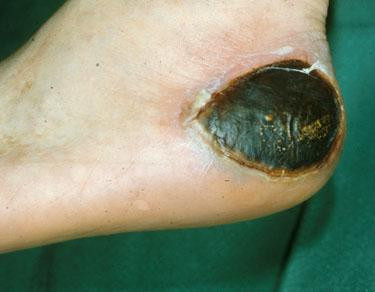
\includegraphics[width=0.7in]{gambar/dataset_citra/luka_hitam/2.jpg}&
		375x292\\
		\hline
		
		& &  &  \\
		2 & 
		luka\_hitam/4.jpg &
		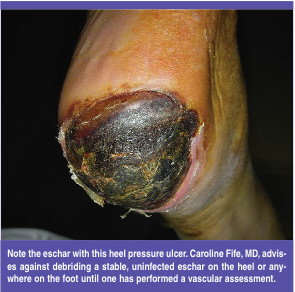
\includegraphics[width=0.7in]{gambar/dataset_citra/luka_hitam/4.jpg}&
		295x292\\
		\hline
		
		& &  &  \\
		3 & 
		luka\_hitam/5.jpg &
		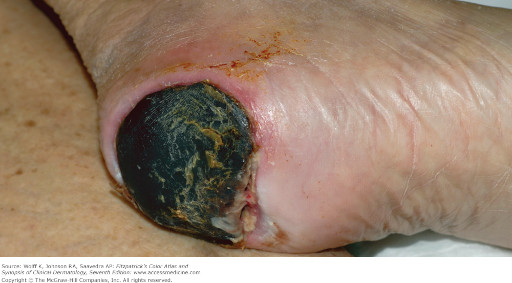
\includegraphics[width=0.7in]{gambar/dataset_citra/luka_hitam/5.jpg}&
		512x283\\
		\hline
		
		& &  &  \\
		4& 
		luka\_hitam/6.jpg &
		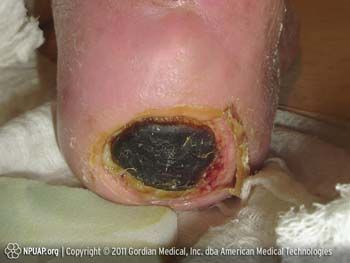
\includegraphics[width=0.7in]{gambar/dataset_citra/luka_hitam/6.jpg}&
		350x263\\
		\hline
		
		& &  &  \\
		5& 
		luka\_hitam/7.jpg &
		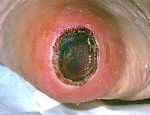
\includegraphics[width=0.7in]{gambar/dataset_citra/luka_hitam/7.jpg}&
		150x115\\
		\hline
		
		& &  &  \\
		6& 
		luka\_hitam/8.jpg &
		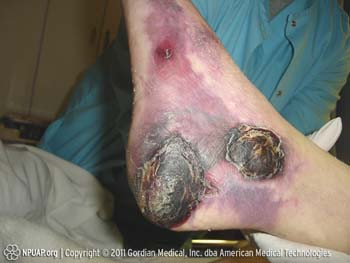
\includegraphics[width=0.7in]{gambar/dataset_citra/luka_hitam/8.jpg}&
		350x263\\
		\hline
		
		& &  &  \\
		7& 
		luka\_hitam/14.jpg &
		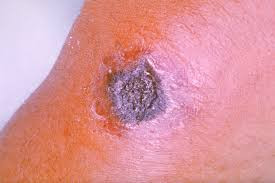
\includegraphics[width=0.7in]{gambar/dataset_citra/luka_hitam/14.jpg}&
		275x183\\
		\hline

		& &  &  \\
		8 & 
		luka\_hitam/15.jpg &
		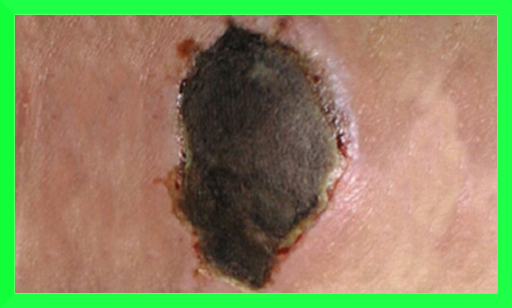
\includegraphics[width=0.7in]{gambar/dataset_citra/luka_hitam/15.jpg}&
		512x308\\
		\hline
		
		& &  &  \\
		9 & 
		luka\_hitam/17.jpg &
		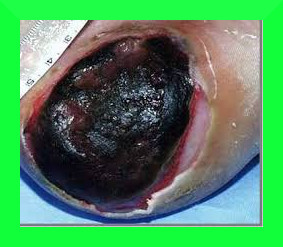
\includegraphics[width=0.7in]{gambar/dataset_citra/luka_hitam/17.jpg}&
		283x247\\
		\hline
	\end{tabular}
\end{table}

\begin{table}[H]
	\centering
	\caption{Visualisasi hasil pengolahan data citra input luka hitam - lanjutan}
	\label{tabel_input_2}
	\begin{tabular}{|m{0.2in}|m{1.2in}|m{0.7in}|m{0.7in}|}
		\hline
		\textbf{No} & \textbf{File} & \textbf{Citra} & \textbf{resolusi} \\
		\hline
		
		& &  &  \\
		10 & 
		luka\_hitam/18.jpg &
		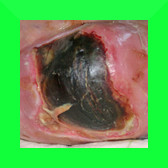
\includegraphics[width=0.7in]{gambar/dataset_citra/luka_hitam/18.jpg}&
		168x168\\
		\hline
		
		& &  &  \\
		11& 
		luka\_hitam/19.jpg &
		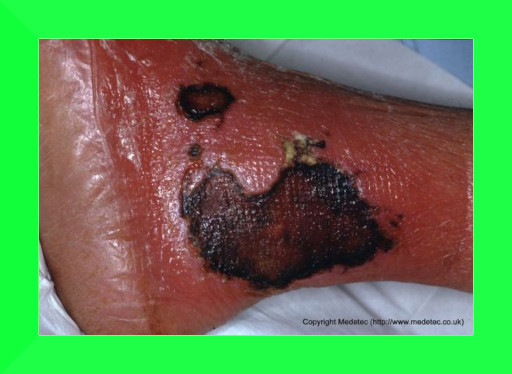
\includegraphics[width=0.7in]{gambar/dataset_citra/luka_hitam/19.jpg}&
		512x374\\
		\hline
		
		& &  &  \\
		12& 
		luka\_hitam/20.jpg &
		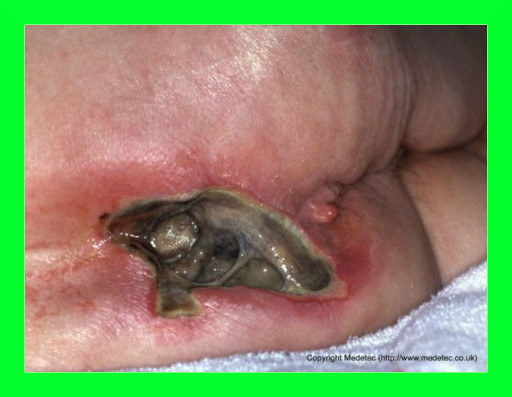
\includegraphics[width=0.7in]{gambar/dataset_citra/luka_hitam/20.jpg}&
		512x397\\
		\hline
		
		& &  &  \\
		13& 
		luka\_hitam/22.jpg &
		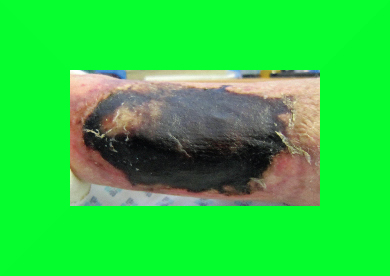
\includegraphics[width=0.7in]{gambar/dataset_citra/luka_hitam/22.jpg}&
		390x276\\
		\hline
		
		& &  &  \\
		14& 
		luka\_hitam/26.jpg &
		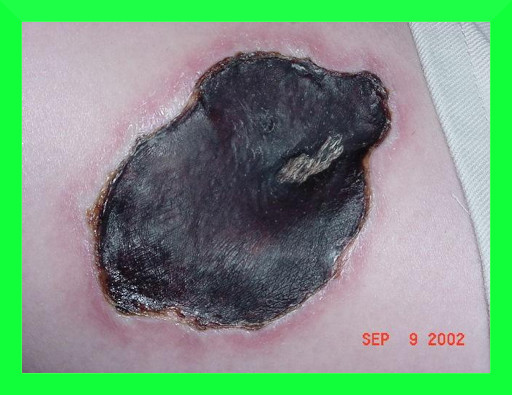
\includegraphics[width=0.7in]{gambar/dataset_citra/luka_hitam/26.jpg}&
		512x395\\
		\hline

		& &  &  \\
		15 & 
		luka\_hitam/27.jpg &
		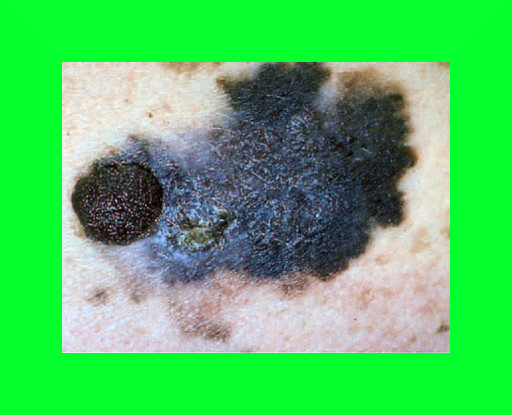
\includegraphics[width=0.7in]{gambar/dataset_citra/luka_hitam/27.jpg}&
		512x415\\
		\hline
		
		& &  &  \\
		16 & 
		luka\_hitam/28.jpg &
		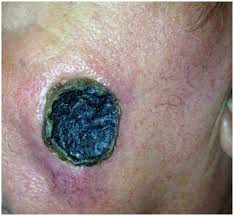
\includegraphics[width=0.7in]{gambar/dataset_citra/luka_hitam/28.jpg}&
		234x216\\
		\hline
		
		& &  &  \\
		17 & 
		luka\_hitam/29.jpg &
		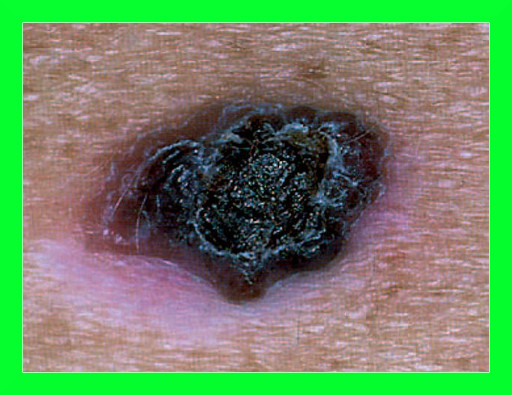
\includegraphics[width=0.7in]{gambar/dataset_citra/luka_hitam/29.jpg}&
		512x395\\
		\hline
	
		& &  &  \\
		18& 
		luka\_hitam/33.jpg &
		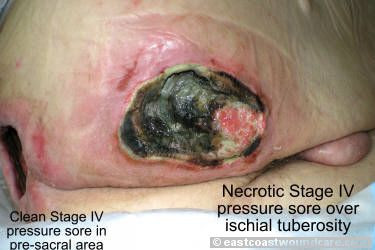
\includegraphics[width=0.7in]{gambar/dataset_citra/luka_hitam/33.jpg}&
		375x250\\
		\hline

	\end{tabular}
\end{table}

\begin{table}[H]
	\centering
	\caption{Visualisasi hasil pengolahan data citra input luka hitam - lanjutan}
	\label{tabel_input_3}
	\begin{tabular}{|m{0.2in}|m{1.2in}|m{0.7in}|m{0.7in}|}
		\hline
		\textbf{No} & \textbf{File} & \textbf{Citra} & \textbf{resolusi} \\
		\hline

		& &  &  \\
		19& 
		luka\_hitam/37.jpg &
		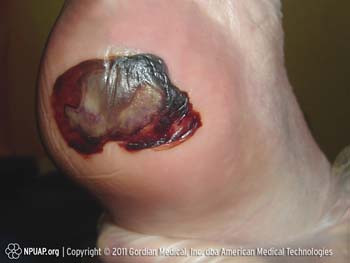
\includegraphics[width=0.7in]{gambar/dataset_citra/luka_hitam/37.jpg}&
		350x263\\
		\hline
		
		& &  &  \\
		20& 
		luka\_hitam/40.jpg &
		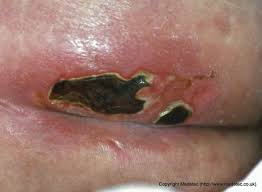
\includegraphics[width=0.7in]{gambar/dataset_citra/luka_hitam/40.jpg}&
		262x192\\
		\hline
		
		& &  &  \\
		21& 
		luka\_hitam/41.jpg &
		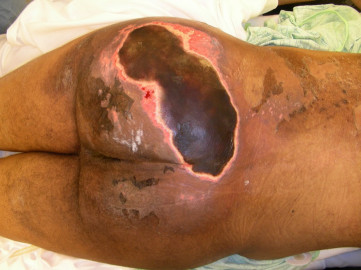
\includegraphics[width=0.7in]{gambar/dataset_citra/luka_hitam/41.jpg}&
		361x270\\
		\hline

		& &  &  \\
		22 & 
		luka\_hitam/16.jpg &
		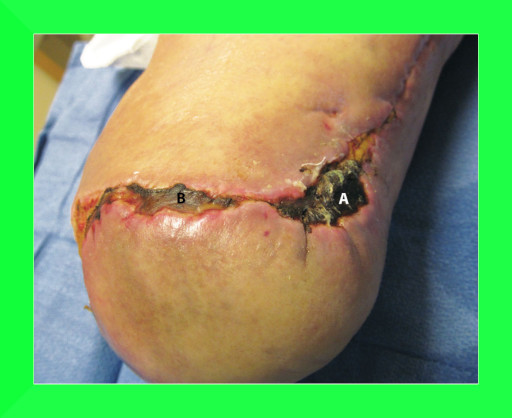
\includegraphics[width=0.7in]{gambar/dataset_citra/luka_hitam/16.jpg}&
		512x418\\
		\hline
		
		& &  &  \\
		23 & 
		luka\_hitam/31.jpg &
		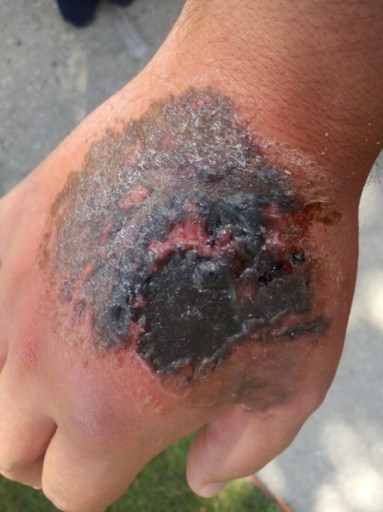
\includegraphics[width=0.7in]{gambar/dataset_citra/luka_hitam/31.jpg}&
		383x512\\
		\hline
		
		& &  &  \\
		24 & 
		luka\_hitam/39.jpg &
		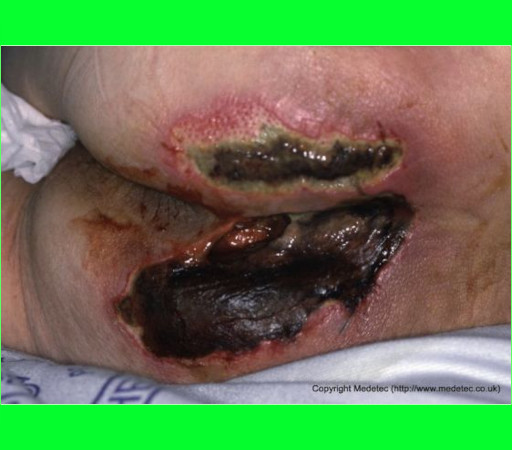
\includegraphics[width=0.7in]{gambar/dataset_citra/luka_hitam/39.jpg}&
		512x450\\
		\hline

	\end{tabular}
\end{table}

\begin{table}[H]
	\centering
	\caption{Visualisasi hasil pengolahan data citra input luka kuning}
	\label{tabel_input_5}
	\begin{tabular}{|m{0.2in}|m{1.2in}|m{0.7in}|m{0.7in}|}
		\hline
		\textbf{No} & \textbf{File} & \textbf{Citra} & \textbf{resolusi} \\
		\hline
		
		& &  &  \\
		1 & 
		luka\_kuning/13.jpg &
		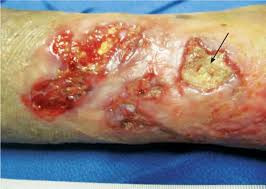
\includegraphics[width=0.7in]{gambar/dataset_citra/luka_kuning/13.jpg}&
		266x189\\
		\hline
		
		& &  &  \\
		2& 
		luka\_kuning/17.jpg &
		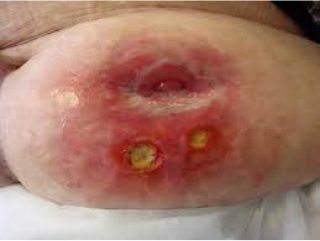
\includegraphics[width=0.7in]{gambar/dataset_citra/luka_kuning/17.jpg}&
		259x194\\
		\hline
		
		& &  &  \\
		3& 
		luka\_kuning/18.jpg &
		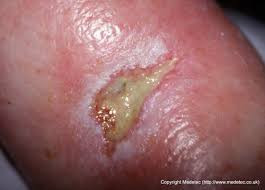
\includegraphics[width=0.7in]{gambar/dataset_citra/luka_kuning/18.jpg}&
		265x190\\
		\hline
		
		& &  &  \\
		4& 
		luka\_kuning/19.jpg &
		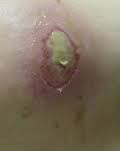
\includegraphics[width=0.7in]{gambar/dataset_citra/luka_kuning/19.jpg}&
		120x151\\
		\hline
		
		& &  &  \\
		5& 
		luka\_kuning/21.jpg &
		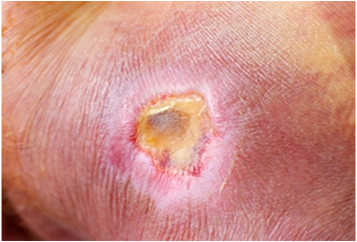
\includegraphics[width=0.7in]{gambar/dataset_citra/luka_kuning/21.jpg}&
		357x242\\
		\hline
		
		& &  &  \\
		6& 
		luka\_kuning/23.jpg &
		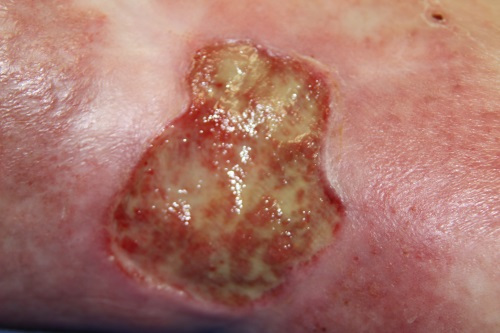
\includegraphics[width=0.7in]{gambar/dataset_citra/luka_kuning/23.jpg}&
		500x333\\
		\hline
		
		& &  &  \\
		7& 
		luka\_kuning/25.jpg &
		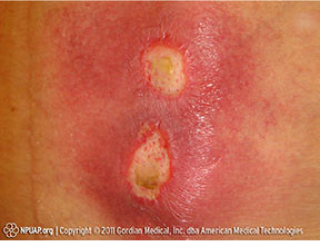
\includegraphics[width=0.7in]{gambar/dataset_citra/luka_kuning/25.jpg}&
		288x216\\
		\hline
				
		& &  &  \\
		8 & 
		luka\_kuning/34.jpg &
		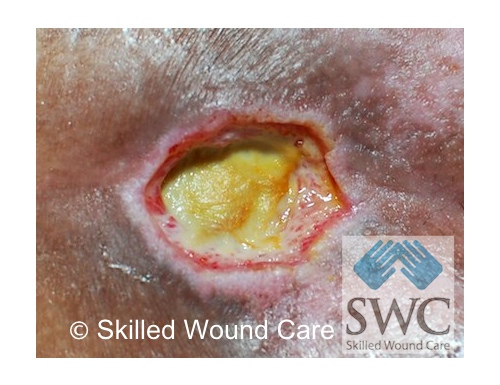
\includegraphics[width=0.7in]{gambar/dataset_citra/luka_kuning/34.jpg}&
		500x385\\
		\hline
		
		& &  &  \\
		9& 
		luka\_kuning/35.jpg &
		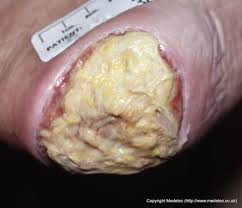
\includegraphics[width=0.7in]{gambar/dataset_citra/luka_kuning/35.jpg}&
		242x208\\
		\hline
		
		& &  &  \\
		10& 
		luka\_kuning/38.jpg &
		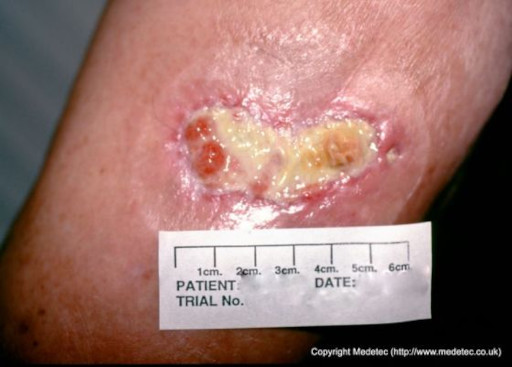
\includegraphics[width=0.7in]{gambar/dataset_citra/luka_kuning/38.jpg}&
		512x367\\
		\hline

	\end{tabular}
\end{table}

\begin{table}[H]
	\centering
	\caption{Visualisasi hasil pengolahan data citra input luka kuning - lanjutan}
	\label{tabel_input_6}
	\begin{tabular}{|m{0.2in}|m{1.2in}|m{0.7in}|m{0.7in}|}
		\hline
		\textbf{No} & \textbf{File} & \textbf{Citra} & \textbf{resolusi} \\
		\hline
		
		& &  &  \\
		11& 
		luka\_kuning/42.jpg &
		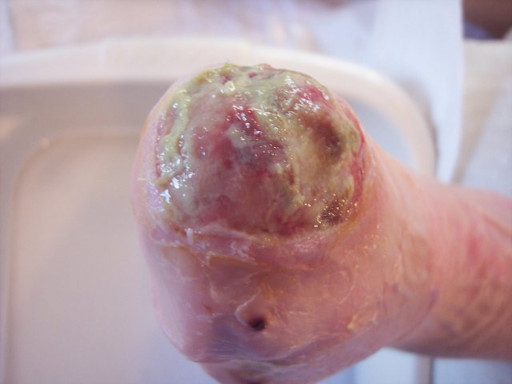
\includegraphics[width=0.7in]{gambar/dataset_citra/luka_kuning/42.jpg}&
		512x384\\
		\hline
		
		& &  &  \\
		12& 
		luka\_kuning/3.jpg &
		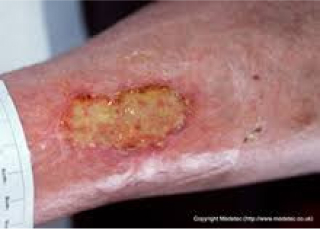
\includegraphics[width=0.7in]{gambar/dataset_citra/luka_kuning/3.jpg}&
		220x157\\
		\hline
		
		& &  &  \\
		13& 
		luka\_kuning/12.jpg &
		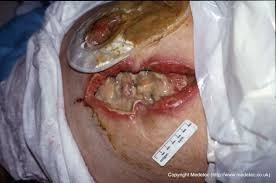
\includegraphics[width=0.7in]{gambar/dataset_citra/luka_kuning/12.jpg}&
		500x333\\
		\hline
		
		& &  &  \\
		14& 
		luka\_kuning/10.jpg &
		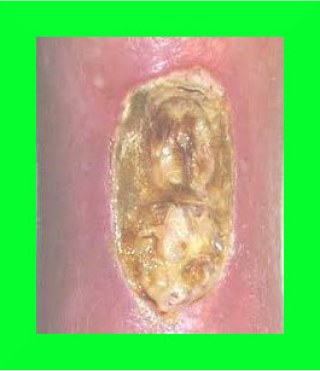
\includegraphics[width=0.7in]{gambar/dataset_citra/luka_kuning/10.jpg}&
		276x183\\
		\hline
				
		& &  &  \\
		15 & 
		luka\_kuning/16.jpg &
		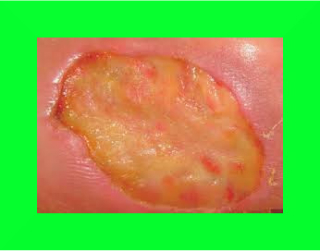
\includegraphics[width=0.7in]{gambar/dataset_citra/luka_kuning/16.jpg}&
		346x270\\
		\hline
	\end{tabular}
\end{table}

\begin{table}[H]
	\centering
	\caption{Visualisasi hasil pengolahan data citra input luka merah}
	\label{tabel_input_8}
	\begin{tabular}{|m{0.2in}|m{1.2in}|m{0.7in}|m{0.7in}|}
		\hline
		\textbf{No} & \textbf{File} & \textbf{Citra} & \textbf{resolusi} \\
		\hline
		
		& &  &  \\
		1 & 
		luka\_merah/16.jpg &
		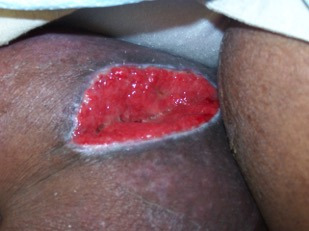
\includegraphics[width=0.7in]{gambar/dataset_citra/luka_merah/16.jpg}&
		309x231\\
		\hline
		
		& &  &  \\
		2& 
		luka\_merah/17.jpg &
		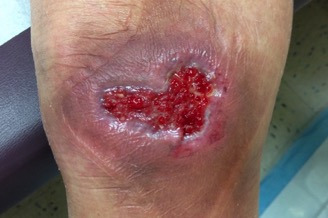
\includegraphics[width=0.7in]{gambar/dataset_citra/luka_merah/17.jpg}&
		328x218\\
		\hline
		
		& &  &  \\
		3& 
		luka\_merah/22.jpg &
		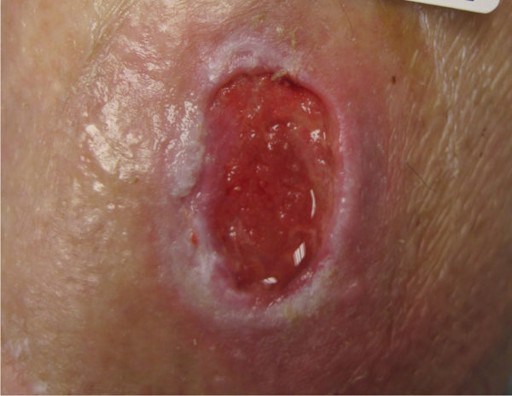
\includegraphics[width=0.7in]{gambar/dataset_citra/luka_merah/22.jpg}&
		512x396\\
		\hline
		
		& &  &  \\
		4& 
		luka\_merah/24.jpg &
		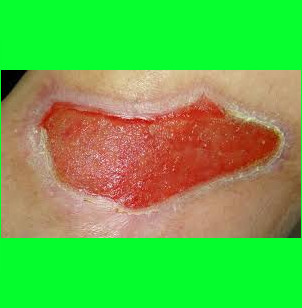
\includegraphics[width=0.7in]{gambar/dataset_citra/luka_merah/24.jpg}&
		302x308\\
		\hline
		
		& &  &  \\
		5& 
		luka\_merah/25.jpg &
		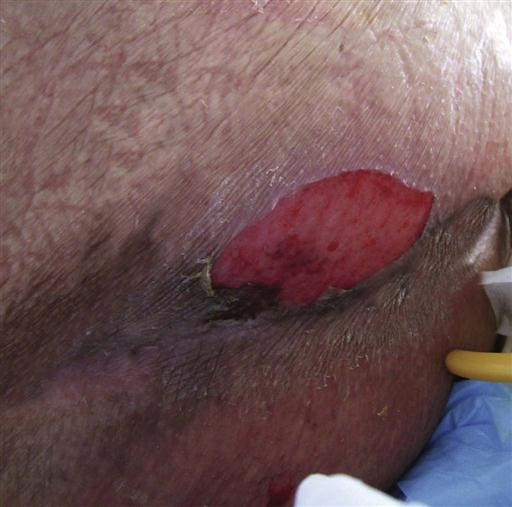
\includegraphics[width=0.7in]{gambar/dataset_citra/luka_merah/25.jpg}&
		512x507\\
		\hline
		
		& &  &  \\
		6& 
		luka\_merah/30.jpg &
		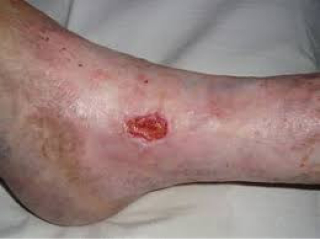
\includegraphics[width=0.7in]{gambar/dataset_citra/luka_merah/30.jpg}&
		260x194\\
		\hline
		
		& &  &  \\
		7& 
		luka\_merah/32.jpg &
		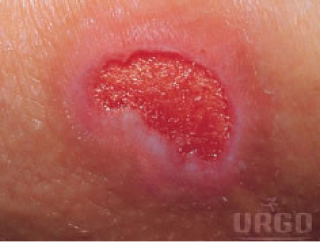
\includegraphics[width=0.7in]{gambar/dataset_citra/luka_merah/32.jpg}&
		236x178\\
		\hline

			
		& &  &  \\
		8 & 
		luka\_merah/33.jpg &
		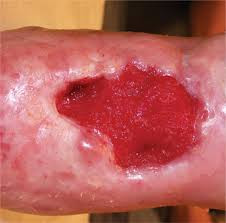
\includegraphics[width=0.7in]{gambar/dataset_citra/luka_merah/33.jpg}&
		226x223\\
		\hline
		
		& &  &  \\
		9& 
		luka\_merah/37.jpg &
		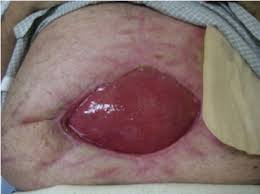
\includegraphics[width=0.7in]{gambar/dataset_citra/luka_merah/37.jpg}&
		260x194\\
		\hline
		
		& &  &  \\
		10& 
		luka\_merah/39.jpg &
		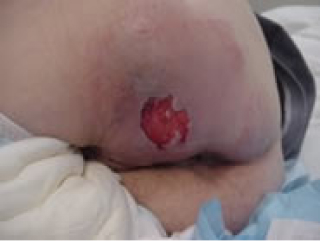
\includegraphics[width=0.7in]{gambar/dataset_citra/luka_merah/39.jpg}&
		185x139\\
		\hline

	\end{tabular}
\end{table}

\begin{table}[H]
	\centering
	\caption{Visualisasi hasil pengolahan data citra input luka merah - lanjutan}
	\label{tabel_input_9}
	\begin{tabular}{|m{0.2in}|m{1.2in}|m{0.7in}|m{0.7in}|}
		\hline
		\textbf{No} & \textbf{File} & \textbf{Citra} & \textbf{resolusi} \\
		\hline
		
		& &  &  \\
		11& 
		luka\_merah/42.jpg &
		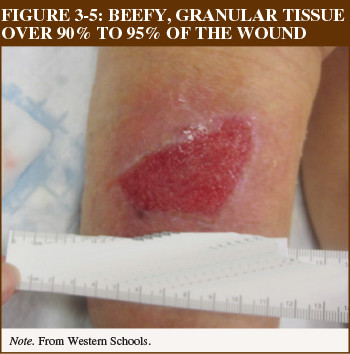
\includegraphics[width=0.7in]{gambar/dataset_citra/luka_merah/42.jpg}&
		350x354\\
		\hline
		
		& &  &  \\
		12& 
		luka\_merah/44.jpg &
		\includegraphics[width=0.7in]{gambar/dataset_citra/luka_merah/44.jpg}&
		512x363\\
		\hline
		
		& &  &  \\
		13& 
		luka\_merah/2.jpg &
		\includegraphics[width=0.7in]{gambar/dataset_citra/luka_merah/2.jpg}&
		288x512\\
		\hline
		
		& &  &  \\
		14& 
		luka\_merah/3.jpg &
		\includegraphics[width=0.7in]{gambar/dataset_citra/luka_merah/3.jpg}&
		384x512\\
		\hline

		& &  &  \\
		15 & 
		luka\_merah/4.jpg &
		\includegraphics[width=0.7in]{gambar/dataset_citra/luka_merah/4.jpg}&
		384x512\\
		\hline
		
		& &  &  \\
		16& 
		luka\_merah/6.jpg &
		\includegraphics[width=0.7in]{gambar/dataset_citra/luka_merah/6.jpg}&
		512x384\\
		\hline
		
		& &  &  \\
		17& 
		luka\_merah/7.jpg &
		\includegraphics[width=0.7in]{gambar/dataset_citra/luka_merah/7.jpg}&
		512x341\\
		\hline
		
		& &  &  \\
		18& 
		luka\_merah/8.jpg &
		\includegraphics[width=0.7in]{gambar/dataset_citra/luka_merah/8.jpg}&
		512x384\\
		\hline
		
	\end{tabular}
\end{table}

\begin{table}[H]
	\centering
	\caption{Visualisasi hasil pengolahan data citra input luka merah - lanjutan}
	\label{tabel_input_10}
	\begin{tabular}{|m{0.2in}|m{1.2in}|m{0.7in}|m{0.7in}|}
		\hline
		\textbf{No} & \textbf{File} & \textbf{Citra} & \textbf{resolusi} \\
		\hline
			
		& &  &  \\
		19& 
		luka\_merah/9.jpg &
		\includegraphics[width=0.7in]{gambar/dataset_citra/luka_merah/9.jpg}&
		288x512\\
		\hline
		
		& &  &  \\
		20& 
		luka\_merah/10.jpg &
		\includegraphics[width=0.7in]{gambar/dataset_citra/luka_merah/10.jpg}&
		512x384\\
		\hline
		
		& &  &  \\
		21& 
		luka\_merah/11.jpg &
		\includegraphics[width=0.7in]{gambar/dataset_citra/luka_merah/11.jpg}&
		512x384\\
		\hline

		& &  &  \\
		22 & 
		luka\_merah/12.jpg &
		\includegraphics[width=0.7in]{gambar/dataset_citra/luka_merah/12.jpg}&
		512x384\\
		\hline
		
		& &  &  \\
		23& 
		luka\_merah/14.jpg &
		\includegraphics[width=0.7in]{gambar/dataset_citra/luka_merah/14.jpg}&
		512x384\\
		\hline
		
		& &  &  \\
		24& 
		luka\_merah/18.jpg &
		\includegraphics[width=0.7in]{gambar/dataset_citra/luka_merah/18.jpg}&
		512x382\\
		\hline
		
		& &  &  \\
		25& 
		luka\_merah/19.jpg &
		\includegraphics[width=0.7in]{gambar/dataset_citra/luka_merah/19.jpg}&
		512x458\\
		\hline
		
		& &  &  \\
		26& 
		luka\_merah/20.jpg &
		\includegraphics[width=0.7in]{gambar/dataset_citra/luka_merah/20.jpg}&
		408x360\\
		\hline

	\end{tabular}
\end{table}

\begin{table}[H]
	\centering
	\caption{Visualisasi hasil pengolahan data citra input luka merah - lanjutan}
	\label{tabel_input_12}
	\begin{tabular}{|m{0.2in}|m{1.2in}|m{0.7in}|m{0.7in}|}
		\hline
		\textbf{No} & \textbf{File} & \textbf{Citra} & \textbf{resolusi} \\
		\hline

		& &  &  \\
		27& 
		luka\_merah/23.jpg &
		\includegraphics[width=0.7in]{gambar/dataset_citra/luka_merah/23.jpg}&
		512x384\\
		\hline
		
		& &  &  \\
		28& 
		luka\_merah/26.jpg &
		\includegraphics[width=0.7in]{gambar/dataset_citra/luka_merah/26.jpg}&
		512x464\\
		\hline
		
		& &  &  \\
		29 & 
		luka\_merah/29.jpg &
		\includegraphics[width=0.7in]{gambar/dataset_citra/luka_merah/29.jpg}&
		328x218\\
		\hline
		
		& &  &  \\
		29& 
		luka\_merah/35.jpg &
		\includegraphics[width=0.7in]{gambar/dataset_citra/luka_merah/35.jpg}&
		261x295\\
		\hline
		
		& &  &  \\
		30& 
		luka\_merah/36.jpg &
		\includegraphics[width=0.7in]{gambar/dataset_citra/luka_merah/36.jpg}&
		295x194\\
		\hline
		
		& &  &  \\
		31& 
		luka\_merah/38.jpg &
		\includegraphics[width=0.7in]{gambar/dataset_citra/luka_merah/38.jpg}&
		512x384\\
		\hline
		
		& &  &  \\
		32& 
		luka\_merah/20.jpg &
		\includegraphics[width=0.7in]{gambar/dataset_citra/luka_merah/20.jpg}&
		408x360\\
		\hline
	\end{tabular}
\end{table}

\chapter{Tabel hasil deteksi keliling luka menggunakan \emph{Grabcut}}
\begin{table}[H]
	\centering
	\caption{Visualisasi hasil deteksi keliling luka menggunakan \emph{Grabcut}}
	\label{tabel_hasil_1}
	\begin{tabular}{|m{1.1in}|m{1.1in}|m{1.1in}|m{1.1in}|m{0.7in}|}
		\hline
		\textbf{Inisialisasi Bounding Box} & \textbf{Hasil Segmentasi} & \textbf{Hasil Citra Referensi} & \textbf{Area Segmentasi} & \textbf{Akurasi} \\
		\hline
		
		&  &  & \\
		\includegraphics[width=1.1in]{gambar/hasil_segmentasi/luka_hitam/image_2_rect.jpg} \fontsize{8}{12}{(153,48,299,158)}&
		\includegraphics[width=1.1in]{gambar/hasil_segmentasi/luka_hitam/result_2.jpg}&
		\includegraphics[width=1.1in]{gambar/hasil_segmentasi/luka_hitam/result_2_cv.jpg}&
		\includegraphics[width=1.1in]{gambar/hasil_segmentasi/luka_hitam/mask_2.jpg}&
		98,1 \% \\
		\hline

		&  &  & \\
		\includegraphics[width=1.1in]{gambar/hasil_segmentasi/luka_hitam/image_4_rect.jpg} \fontsize{8}{12}{(60, 89, 162, 153)}&
		\includegraphics[width=1.1in]{gambar/hasil_segmentasi/luka_hitam/result_4.jpg}&
		\includegraphics[width=1.1in]{gambar/hasil_segmentasi/luka_hitam/result_4_cv.jpg}&
		\includegraphics[width=1.1in]{gambar/hasil_segmentasi/luka_hitam/mask_4.jpg}&
		93.3 \% \\
		\hline
		
		&  &  & \\
		\includegraphics[width=1.1in]{gambar/hasil_segmentasi/luka_hitam/image_5_rect.jpg} \fontsize{8}{12}{(68, 48, 115, 106)}&
		\includegraphics[width=1.1in]{gambar/hasil_segmentasi/luka_hitam/result_5.jpg}&
		\includegraphics[width=1.1in]{gambar/hasil_segmentasi/luka_hitam/result_5_cv.jpg}&
		\includegraphics[width=1.1in]{gambar/hasil_segmentasi/luka_hitam/mask_5.jpg}&
		98.0 \% \\
		\hline
		
		&  &  & \\
		\includegraphics[width=1.1in]{gambar/hasil_segmentasi/luka_hitam/image_6_rect.jpg} \fontsize{8}{12}{(83, 97, 130, 97)}&
		\includegraphics[width=1.1in]{gambar/hasil_segmentasi/luka_hitam/result_6.jpg}&
		\includegraphics[width=1.1in]{gambar/hasil_segmentasi/luka_hitam/result_6_cv.jpg}&
		\includegraphics[width=1.1in]{gambar/hasil_segmentasi/luka_hitam/mask_6.jpg}&
		99,6 \% \\
		\hline
		
		&  &  & \\
		\includegraphics[width=1.1in]{gambar/hasil_segmentasi/luka_hitam/image_7_rect.jpg} \fontsize{8}{12}{(100, 50, 117, 142)}&
		\includegraphics[width=1.1in]{gambar/hasil_segmentasi/luka_hitam/result_7.jpg}&
		\includegraphics[width=1.1in]{gambar/hasil_segmentasi/luka_hitam/result_7_cv.jpg}&
		\includegraphics[width=1.1in]{gambar/hasil_segmentasi/luka_hitam/mask_7.jpg}&
		99,4 \% \\
		\hline
	\end{tabular}
\end{table}

\begin{table}[H]
	\centering
	\caption{Visualisasi hasil deteksi keliling luka menggunakan \emph{Grabcut}}
	\label{tabel_hasil_2}
	\begin{tabular}{|m{1.1in}|m{1.1in}|m{1.1in}|m{1.1in}|m{0.7in}|}
		\hline
		\textbf{Inisialisasi Bounding Box} & \textbf{Hasil Segmentasi} & \textbf{Hasil Citra Referensi} & \textbf{Area Segmentasi} & \textbf{Akurasi} \\
		\hline
		
		&  &  & \\
		\includegraphics[width=1.1in]{gambar/hasil_segmentasi/luka_hitam/image_8_rect.jpg} \fontsize{8}{12}{(114, 104, 157, 108)}&
		\includegraphics[width=1.1in]{gambar/hasil_segmentasi/luka_hitam/result_8.jpg}&
		\includegraphics[width=1.1in]{gambar/hasil_segmentasi/luka_hitam/result_8_cv.jpg}&
		\includegraphics[width=1.1in]{gambar/hasil_segmentasi/luka_hitam/mask_8.jpg}&
		64,4 \% \\
		\hline
		
		&  &  & \\
		\includegraphics[width=1.1in]{gambar/hasil_segmentasi/luka_hitam/image_14_rect.jpg} \fontsize{8}{12}{(98, 43, 116, 121)}&
		\includegraphics[width=1.1in]{gambar/hasil_segmentasi/luka_hitam/result_14.jpg}&
		\includegraphics[width=1.1in]{gambar/hasil_segmentasi/luka_hitam/result_14_cv.jpg}&
		\includegraphics[width=1.1in]{gambar/hasil_segmentasi/luka_hitam/mask_14.jpg}&
		90,6 \% \\
		\hline
		
		&  &  & \\
		\includegraphics[width=1.1in]{gambar/hasil_segmentasi/luka_hitam/image_15_rect.jpg} \fontsize{8}{12}{(89, 10, 140, 171)}&
		\includegraphics[width=1.1in]{gambar/hasil_segmentasi/luka_hitam/result_15.jpg}&
		\includegraphics[width=1.1in]{gambar/hasil_segmentasi/luka_hitam/result_15_cv.jpg}&
		\includegraphics[width=1.1in]{gambar/hasil_segmentasi/luka_hitam/mask_15.jpg}&
		95,7 \% \\
		\hline
		
		&  &  & \\
		\includegraphics[width=1.1in]{gambar/hasil_segmentasi/luka_hitam/image_17_rect.jpg} \fontsize{8}{12}{(28, 34, 208, 213)}&
		\includegraphics[width=1.1in]{gambar/hasil_segmentasi/luka_hitam/result_17.jpg}&
		\includegraphics[width=1.1in]{gambar/hasil_segmentasi/luka_hitam/result_17_cv.jpg}&
		\includegraphics[width=1.1in]{gambar/hasil_segmentasi/luka_hitam/mask_17.jpg}&
		90,3 \% \\
		\hline
		
		&  &  & \\
		\includegraphics[width=1.1in]{gambar/hasil_segmentasi/luka_hitam/image_18_rect.jpg} \fontsize{8}{12}{(50, 59, 219, 201)}&
		\includegraphics[width=1.1in]{gambar/hasil_segmentasi/luka_hitam/result_18.jpg}&
		\includegraphics[width=1.1in]{gambar/hasil_segmentasi/luka_hitam/result_18_cv.jpg}&
		\includegraphics[width=1.1in]{gambar/hasil_segmentasi/luka_hitam/mask_18.jpg}&
		88,1 \% \\
		\hline

	\end{tabular}
\end{table}


\begin{table}[H]
	\centering
	\caption{Visualisasi hasil deteksi keliling luka menggunakan \emph{Grabcut}}
	\label{tabel_hasil_3}
	\begin{tabular}{|m{1.1in}|m{1.1in}|m{1.1in}|m{1.1in}|m{0.7in}|}
		\hline
		\textbf{Inisialisasi Bounding Box} & \textbf{Hasil Segmentasi} & \textbf{Hasil Citra Referensi} & \textbf{Area Segmentasi} & \textbf{Akurasi} \\
		\hline

		&  &  & \\
		\includegraphics[width=1.1in]{gambar/hasil_segmentasi/luka_hitam/image_19_rect.jpg} \fontsize{8}{12}{(107, 82, 147, 104)}&
		\includegraphics[width=1.1in]{gambar/hasil_segmentasi/luka_hitam/result_19.jpg}&
		\includegraphics[width=1.1in]{gambar/hasil_segmentasi/luka_hitam/result_19_cv.jpg}&
		\includegraphics[width=1.1in]{gambar/hasil_segmentasi/luka_hitam/mask_19.jpg}&
		97.6 \% \\
		\hline
		
		&  &  & \\
		\includegraphics[width=1.1in]{gambar/hasil_segmentasi/luka_hitam/image_20_rect.jpg} \fontsize{8}{12}{(51, 107, 168, 101)}&
		\includegraphics[width=1.1in]{gambar/hasil_segmentasi/luka_hitam/result_20.jpg}&
		\includegraphics[width=1.1in]{gambar/hasil_segmentasi/luka_hitam/result_20_cv.jpg}&
		\includegraphics[width=1.1in]{gambar/hasil_segmentasi/luka_hitam/mask_20.jpg}&
		82,9 \% \\
		\hline
		
		&  &  & \\
		\includegraphics[width=1.1in]{gambar/hasil_segmentasi/luka_hitam/image_22_rect.jpg} \fontsize{8}{12}{(63, 67, 186, 98)}&
		\includegraphics[width=1.1in]{gambar/hasil_segmentasi/luka_hitam/result_22.jpg}&
		\includegraphics[width=1.1in]{gambar/hasil_segmentasi/luka_hitam/result_22_cv.jpg}&
		\includegraphics[width=1.1in]{gambar/hasil_segmentasi/luka_hitam/mask_22.jpg}&
		85,2 \% \\
		\hline
		
	\end{tabular}
\end{table}